\documentclass[12pt]{report}

\def\MakeUppercaseUnsupportedInPdfStrings{\scshape}

\usepackage{listings, titling}
\usepackage{color}
\usepackage{graphicx}
\usepackage{hyperref}
\usepackage{biblatex}
\usepackage{float}
\graphicspath{ {./images/} }
\definecolor{dkgreen}{rgb}{0,0.6,0}
\definecolor{gray}{rgb}{0.5,0.5,0.5}
\definecolor{mauve}{rgb}{0.58,0,0.82}

\lstset{frame=tb,
	language=C,
	aboveskip=3mm,
	belowskip=3mm,
	showstringspaces=false,
	columns=flexible,
	basicstyle={\small\ttfamily},
	numbers=none,
	numberstyle=\tiny\color{gray},
	keywordstyle=\color{blue},
	commentstyle=\color{gray},
	stringstyle=\color{mauve},
	breaklines=true,
	breakatwhitespace=true,
	tabsize=3
}

% Title Page
\newcommand*{\myTitle}{\begingroup 
	\centering 
	\vspace*{\baselineskip} 
	
	
	{\LARGE Advanced Operating Systems}% Title
	\vspace*{1\baselineskip}
	
	\scshape % Small caps
	Multi-flow device file
	
	\vspace*{1\baselineskip}
	University of Rome Tor Vergata\\[\baselineskip]
	
	
	\vspace*{5\baselineskip} 
	
	{\large Di Battista Mattia (0304938)\par} 
	
	\vspace*{1\baselineskip}
	\today
	
	\endgroup\clearpage}

\begin{document}
\begin{titlingpage}
\myTitle
\end{titlingpage}
\tableofcontents

\chapter{Specification}

This specification is related to a Linux device driver implementing low and high priority flows of data.
Through an open session to the device file a thread can read/write data segments. The data delivery
follows a First-in-First-out policy along each of the two different data flows (low and high priority). After
read operations, the read data disappear from the flow. Also, the high priority data flow must offer
synchronous write operations while the low priority data flow must offer an asynchronous execution
(based on delayed work) of write operations, while still keeping the interface able to synchronously notify
the outcome. Read operations are all executed synchronously. The device driver should support 128
devices corresponding to the same amount of minor numbers.

The device driver should implement the support for the \emph{ioctl(..)} service in order to manage the I/O session
as follows:
\begin{itemize}
\item setup of the priority level (high or low) for the operations
\item blocking vs non-blocking read and write operations
\item setup of a timeout regulating the awake of blocking operations
\end{itemize}

A few Linux module parameters and functions should be implemented in order to enable or disable the
device file, in terms of a specific minor number. If it is disabled, any attempt to open a session should fail
(but already open sessions will be still managed). Further additional parameters exposed via VFS should
provide a picture of the current state of the device according to the following information:
\begin{itemize}
\item enabled or disabled
\item number of bytes currently present in the two flows (high vs low priority)
\item number of threads currently waiting for data along the two flows (high vs low priority)
\end{itemize}

\chapter{Operations}
\section{Setting Operation}

The user can set four modes of operation for his working session: 

\begin{enumerate}
	\itemsep0em 
	\item low priority
	\item high priority
	\item blocking
	\item non blocking
\end{enumerate}

The data structure to store these parameters is:

\begin{lstlisting}
//FILE: info.h
typedef struct _session{
	bool priority;       
	bool blocking;
	unsigned long timeout;
} session;
\end{lstlisting}

It is unique for each thread, unlike the \emph{\_object\_state} defined for every device file.

\begin{lstlisting}
//FILE: info.h
typedef struct _object_state{
	struct mutex operation_synchronizer;
	memory_node *head;
	wait_queue_head_t wq;
} object_state;
\end{lstlisting}

\emph{\_\_session} is instantiated in \emph{dev\_open()}:

\begin{lstlisting}
//FILE: multi_flow.c
session = kmalloc(sizeof(session), GFP_KERNEL);
//...
if (session == NULL) //...
session->priority = HIGH_PRIORITY;
session->blocking = NON_BLOCKING;
session->timeout = 0;
file->private_data = session;
\end{lstlisting}

The field \emph{unsigned long timeout} indicates the maximum time (expressed as microseconds) awaited in blocking operations (see Sec. \ref{chap:blocking operation}). 

Parameter setting is done within \emph{dev\_ioctl()}:

\begin{lstlisting}
//FILE: multi_flow.c
static long dev_ioctl(struct file *filp, 
	unsigned int command, 
	unsigned long param){

	session *session;
	session = filp->private_data;
	
	switch (command){
	case 3:
		session->priority = LOW_PRIORITY;
		//...
		break;
	//...
	case 7:
		session->timeout = param;
		//...
		break;
	//...
}
\end{lstlisting}

To associate the session to a user, the field \emph{private\_data} of \emph{struct file *filp} has been used. 

\section{Blocking Operation}
\label{chap:blocking operation}
For blocking operations the thread goes to sleep, in the respective wait queue of the object\footnote{There are  two for each object: a low and high priority queue.}, in case it fails to take the lock. 

\begin{lstlisting}
//FILE: common.h
static int blocking(unsigned long timeout, struct mutex *mutex, wait_queue_head_t *wq){
	//...	
	timeout = msecs_to_jiffies(timeout); 	
	//Returns 0, if the condition evaluated to false after the timeout elapsed
	val = wait_event_timeout(*wq, mutex_trylock(mutex), timeout);
	//...
}
\end{lstlisting}

To wake all threads sleeping on the given wait queue, \emph{wake\_up()} is invoked at the end of every operations (after having released the lock). 

Threads wait for a certain time, until the lock is released. Time passed to \emph{wait\_event\_timeout()} is converted from microseconds to jiffies with \emph{msecs\_to\_jiffies()}. An error code\footnote{EAGAIN: Resource temporarily unavailable.} is returned if the timer has expired.

\section{Write Operation}
\label{chap:write operation}

Unlike read operations (see Sec. \ref{chap:read operation}), write can be done with low priority (based on delayed work). In this way the operation is performed by system daemons\footnote{Work queues allow you to queue blocking activities, executed by threads in charge of doing this.}.

\begin{lstlisting}
//FILE: multi_flow.c
if (session->priority == HIGH_PRIORITY){
	priority_obj = &the_object[HIGH_PRIORITY];
	//...	
	ret = write(priority_obj, buff, off, len, session, minor);
}else{
	priority_obj = &the_object[LOW_PRIORITY];
	//...	
	ret = put_work(filp, buff, len, off, priority_obj, session, minor);
	if (ret != 0) //...
	ret = len;
}
\end{lstlisting}

To define deferred work:

\begin{lstlisting}
//FILE: write.h
long put_work(struct file *filp,
	const char *buff,
	size_t len,
	loff_t *off,
	object_state *the_object,
	session *session,
	int minor){
	
	//...
	
	__INIT_WORK(&(the_task->the_work), (void *)delayed_write, (unsigned long)(&(the_task->the_work)));
	
	schedule_work(&the_task->the_work);
	
	return 0;
}
\end{lstlisting}

For each write operation a new \emph{memory\_node} (see Sec. \ref{chap:read operation}) and buffer (both with \emph{kmalloc()}\footnote{This API allows to reserve Bytes and not whole pages like \emph{get\_free\_page()}.}) are allocated. The buffer's size is equal to the amount of Bytes written from the user. Finally the new node is added to a list (one for every stream). See Image \ref{fig:write}.

\emph{copy\_from\_user()} may sleep if pagefaults are enabled. That's why it is invoked before requiring the lock on the flow\footnote{An alternative could be to invoke \emph{\_\_copy\_to\_user\_inatomic()} (see \href{https://www.kernel.org/doc/htmldocs/kernel-api/API---copy-to-user-inatomic.html}{https://www.kernel.org/doc/htmldocs/kernel-api/API---copy-to-user-inatomic.html})}.

\begin{lstlisting}
//FILE: write.h
int write(object_state *the_object,
	const char *buff,
	loff_t *off, 
	size_t len, 
	session *session,
	int minor){

	//...
	node = kmalloc(sizeof(memory_node), GFP_ATOMIC);
	buffer = kmalloc(len, GFP_ATOMIC);
	if (node == NULL || buffer == NULL){
		printk("%s: unable to allocate a memory\n", MODNAME);
		return -ENOMEM;
	}
	
	ret = copy_from_user(buffer, buff, len);
	
	wq = get_lock(the_object, session, minor);
	if (wq == NULL) return -EAGAIN;
	//...
\end{lstlisting}

\begin{figure}[H]
\label{fig:write}
	\centering
	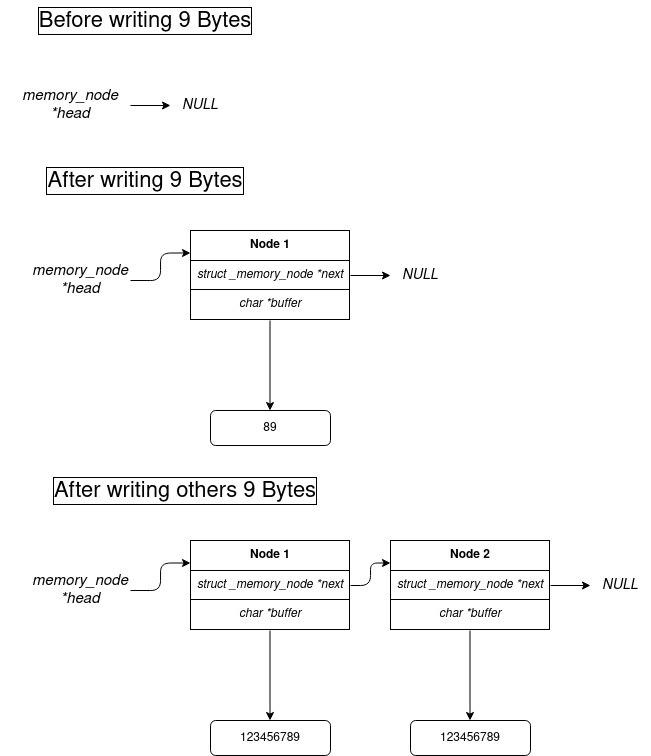
\includegraphics[scale = .45]{write.jpg}
	\caption{Example of write operation}
	\label{fig:write}
\end{figure}

\section{Read Operation}
\label{chap:read operation}

Read operations are all performed synchronously (without delayed work as for write op.). When an invocation occurs the data structure for one of the two flows is set:

\begin{lstlisting}
//FILE: multi_flow.c
if (session->priority == HIGH_PRIORITY){
	priority_obj = &the_object[HIGH_PRIORITY];	
	//...
}else{
	priority_obj = &the_object[LOW_PRIORITY];
	//...
}
ret = read(priority_obj, buff, off, len, session, minor);
\end{lstlisting}

In addition, they involved deleting bytes read by the user, on the current flow. To do this a linked list was used, in which each node keeps the following fields:

\begin{lstlisting}
//FILE: info.h
typedef struct _memory_node{
	char *buffer;
	struct _memory_node *next;
} memory_node;
\end{lstlisting}

Each node points to its own buffer, the size of which can then be different for all items. Buffers are allocated in write operations (see Sec. \ref{chap:write operation}). If the user requests the reading of a smaller number of bytes, than those written on all nodes, the deletion happens for the only read bytes, not on the entire buffer (see Fig. \ref{fig:read}). Reading and deletion begin from the first node (\textbf{First-in-First-out policy}). 

\begin{figure}[h]
	\centering
	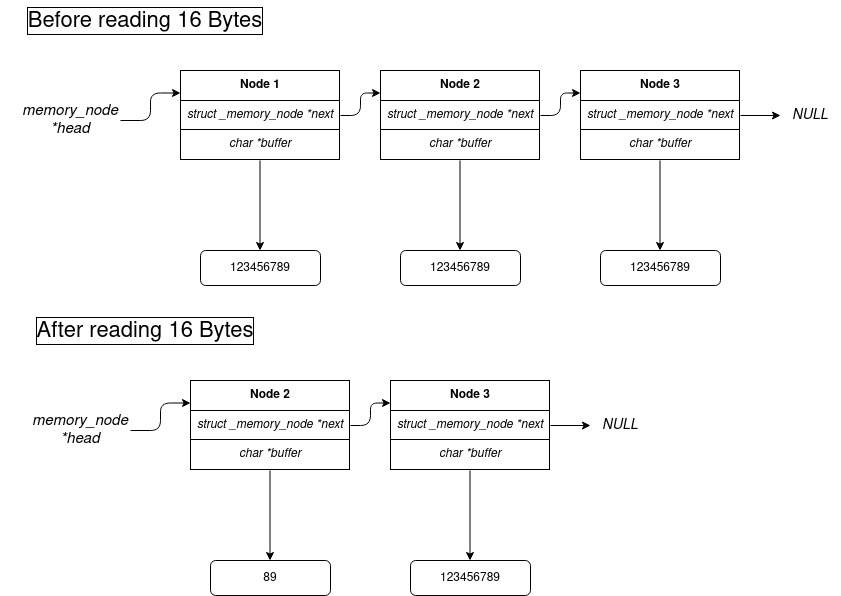
\includegraphics[scale = .45]{read.jpg}
	\caption{Example of read operation}
	\label{fig:read}
\end{figure}

The procedures for doing this are:

\begin{lstlisting}
//FILE: read.h
memory_node *shift_buffer(int, int, memory_node *);
int read(object_state *, const char *, loff_t *, size_t, session *, int);
\end{lstlisting}

\chapter{Parameters}

The required module parameters to deploy are:

\begin{enumerate}
	\itemsep0em 
	\item enable or disable the device file
	\item number of bytes currently present in the two flows (high vs low priority)
	\item number of threads currently waiting for data along the two flows (high vs low priority)
\end{enumerate}

Implemented with:

\begin{lstlisting}
//FILE: info.h
static int enabled_device[MINORS];
module_param_array(enabled_device, int, NULL, 0660);
MODULE_PARM_DESC(...);

static int hp_bytes[MINORS];
module_param_array(hp_bytes, int, NULL, 0660);
MODULE_PARM_DESC(...);

static int lp_bytes[MINORS];
module_param_array(lp_bytes, int, NULL, 0660);
MODULE_PARM_DESC(...);

static int hp_threads[MINORS];
module_param_array(hp_threads, int, NULL, 0660);
MODULE_PARM_DESC(...);

static int lp_threads[MINORS];
module_param_array(lp_threads, int, NULL, 0660);
MODULE_PARM_DESC(...);
\end{lstlisting}
\chapter{How To Use}

Commands for kernel module (in \emph{/code/}): 

\begin{lstlisting}[language=Bash]
#Compile kernel module (on /multi_flow/code/)
make all

#Clean objects file
make clean

#Insertion kernel module
sudo insmod multi_flow.ko

#Remove kernel module
sudo rmmod multi_flow.ko
\end{lstlisting}

Commands for parameters (in \emph{/code/}): 

\begin{lstlisting}[language=Bash]
#Show kernel module's parameters (i.e. enabled_device, hp_bytes, lp_bytes, hp_threads, lp_threads)
make show-device
make show-hp_bytes
make show-lp_bytes
make show-hp_threads
make show-lp_threads
\end{lstlisting}

Commands for user (in \emph{/code/user}): 

\begin{lstlisting}[language=Bash]
#Compile user
make

#Run user 
sudo ./user /dev/test 240 1

#Disable a list of devices by index
sudo python3 script.py 0 1 2 45 127
\end{lstlisting}

To test blocking operations a macro is defined: 

\begin{lstlisting}
//FILE: info.h
#define TEST
\end{lstlisting}

\emph{TEST} does not release the lock after a write, and does not wake up the  threads in the wait queue. 

\begin{lstlisting}
//FILE write.c
#ifndef TEST   
	mutex_unlock(&(the_object->operation_synchronizer));
	wake_up(wq);
#endif
\end{lstlisting}


\end{document}          
